\documentclass[11pt]{article}
\usepackage{fullpage}
\usepackage{amsthm}
\usepackage{amsmath}
\usepackage{amssymb}
\usepackage{graphicx}

\graphicspath{ {./imgs/} }

\setlength{\parindent}{0pt}

\title{Robotics (CO333)}
\author{Michael Tsang}

\newtheorem{defn}{Definition}
\newtheorem{eg}{Example}
\newtheorem{theo}{Theorem}
\newtheorem{lem}{Lemma}

\begin{document}

\maketitle

\section{Robot Motion}
A mobile robot can move and sense, and must process information to link these two.

What are the possible goals of a robot locomotion system?
\begin{itemize}
  \item Speed and/or acceleration of movement.
  \item Precision of positioning (repeatability).
  \item Flexibility and robustness in different conditions.
  \item Efficiency.
\end{itemize}

Robots could move in water, air, land, or even space.
We focus on wheeled robots which move on fairly flat surfaces.

\subsection{Motion and Coordinate Frames}
We define two coordinate frames: a \textbf{world frame} $W$ anchored in the world and a \textbf{robot frame} $R$ which is carried by and stays fixed relative to the robot at all times.

We are interested in the robot's \textbf{location}: the transformation between $W$ and $R$.

\subsection{Degrees of Motion Freedom}
A rigid body which translates and rotates along a:
\begin{itemize}
  \item 1D path has 1 degree of freedom (DOF): 1 translational.
  \item 2D plane has 3 DOF: 2 translational, 1 rotational.
  \item 3D volume has 6 DOF: 3 translational, 3 rotational.
\end{itemize}

A \textbf{holonomic robot} is one which is able to move instantaneously in any direction in the space of its degrees of freedom.

Although holonomic robots exist, they need many motors or unusual designs, and are often impractical.

\subsection{Wheel Configurations}
\begin{itemize}
  \item Rack and Pinion.
  \item Differential Drive.
  \item Skid-Steer.
  \item Synchro Drive.
\end{itemize}
These are standard non-holonomic configurations and are simple, reliable, robust mechanisms suitable for robots which essentially move in a plane.

Some more exotic non-holonomic configurations are:
\begin{itemize}
  \item Segway - good height with small footprint and high acceleration; self balancing.
  \item Mars Rover - wheels on stalks to tackle large obstacles.
\end{itemize}

\subsection{Differential Drive}
\begin{itemize}
  \item Two motors, one per wheel.
  \item Steer by setting different speeds on each wheel.
  \item Wheels run at equal speeds for straight-line motion.
  \item Wheels run at equal and opposite speeds to turn on the spot.
  \item Other combinations of speeds allow circular arcs.
\end{itemize}

\subsection{Circular Path of a Differential Drive Robot}
\begin{figure}[h]
  \caption{Differential Drive Robot}
  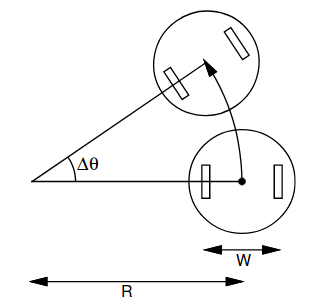
\includegraphics[scale=0.4]{ddrobot}
  \centering
\end{figure}

Let the wheel velocities of the left and right wheels respectively be $v_L$ and $v_R$.
These are linear velocities of the wheels over the ground: $v_X = r_X\omega_X$, where $r_X$ is the radius of the $X$ wheel and $\omega_X$ is its angular velocity.

The width between the wheels is $W$.

\begin{itemize}
  \item Straight line motion if $v_L = v_R$.
  \item Turns on the spot if $v_L = - v_R$.
\end{itemize}

To find radius $R$ of a curved path, consider a period of motion $\Delta t$ where the robot moves along a circular arc through angle $\Delta \theta$.
\begin{itemize}
  \item Left wheel: $\text{distance moved } = v_L \Delta t$; $\text{radius of arc } = R - \frac{W}{2}$.
  \item Right wheel: $\text{distance moved } = v_R \Delta t$; $\text{radius of arc } = R + \frac{W}{2}$.
  \item Both wheel arcs subtend the same angle so:
    \[
      \Delta \theta = \frac{v_L \Delta t}{R - \frac{W}{2}} = \frac{v_R \Delta t}{R + \frac{W}{2}}
    \]
    \[
      \implies \frac{W}{2}(v_L + v_R) = R(v_R - v_L)
    \]
    \begin{align*}
      \implies R &= \frac{W(v_R + v_L)}{2(v_R - v_L)} & \Delta \theta &= \frac{(v_R - v_L)\Delta t}{W}
    \end{align*}
\end{itemize}

\subsection{Rack and Pinion Drive (Car/Tricycle)}
\begin{figure}[h]
  \caption{Rack and Pinion Drive layouts.}
  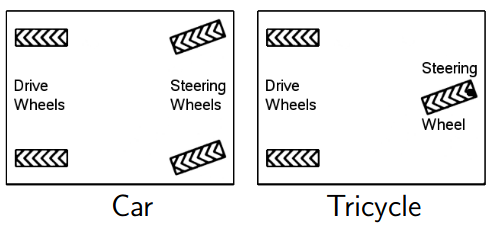
\includegraphics[scale=0.4]{piniondrive}
  \centering
\end{figure}

\begin{itemize}
  \item Two motors: one to drive, one to steer.
  \item Cannot normally turn on the spot.
  \item With fixed speed and steering angle, will follow a circular path.
  \item With four wheels, need rear differential and variable (``Ackerman'') linkage for steering wheels.
\end{itemize}

\subsection{Circular Path of a Car-Like Tricycle Robot}
\begin{figure}[h]
  \caption{Tricycle Robot.}
  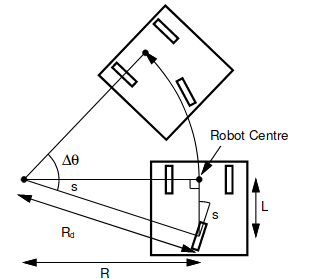
\includegraphics[scale=0.4]{tricycle}
  \centering
\end{figure}

Single steerable and drivable wheel at back, front wheels are free running.

Assuming no sideways wheel slip, we intersect the axes of the front and back wheels to forma right-angle triangle:
\[
  R = \frac{L}{\tan s}
\]

The radius of the path the rear wheels moves is:
\[
  R_d = \frac{L}{\sin s}
\]

In time $\Delta t$, the distance along its circular arc moved by the wheel is $v\Delta t$, so the angle $\Delta \theta$ through which the robot rotates is:
\[
  \Delta \theta = \frac{v\Delta t}{R_d} = \frac{v\Delta t \sin s}{L}
\]


\end{document}

